\documentclass[12pt,letterpaper]{article}
\usepackage{natbib}

%Packages
\usepackage{xcolor}
\usepackage{color,soul}
\usepackage{pdflscape}
\usepackage{fixltx2e}
\usepackage{textcomp}
\usepackage{fullpage}
\usepackage{float}
\usepackage{latexsym}
\usepackage{url}
\usepackage{epsfig}
\usepackage{graphicx}
\usepackage{amssymb}
\usepackage{amsmath}
\usepackage{bm}
\usepackage{array}
\usepackage[version=3]{mhchem}
\usepackage{ifthen}
\usepackage{caption}
\usepackage{hyperref}
\usepackage{amsthm}
\usepackage{amstext}
\usepackage{enumerate}
\usepackage[osf]{mathpazo}
\usepackage{dcolumn}
\usepackage{lineno}
\usepackage{dcolumn}
\usepackage{hyphenat}
\usepackage[T1]{fontenc}
\usepackage{textcomp}
\newcolumntype{d}[1]{D{.}{.}{#1}}

\pagenumbering{arabic}


%Pagination style and stuff
\linespread{2}
\raggedright
\setlength{\parindent}{0.5in}
\setcounter{secnumdepth}{0} 
\renewcommand{\section}[1]{%
\bigskip
\begin{center}
\begin{Large}
\normalfont\scshape #1
\medskip
\end{Large}
\end{center}}
\renewcommand{\subsection}[1]{%
\bigskip
\begin{center}
\begin{large}
\normalfont\itshape #1
\end{large}
\end{center}}
\renewcommand{\subsubsection}[1]{%
\vspace{2ex}
\noindent
\textit{#1.}---}
\renewcommand{\tableofcontents}{}
%\bibpunct{(}{)}{;}{a}{}{,}

%---------------------------------------------
%
%       START
%
%---------------------------------------------

\begin{document}

%Running head
\begin{flushright}
Version dated: \today
\end{flushright}
\bigskip
\noindent RH: disparate views on disparity.

\bigskip
\medskip
\begin{center}

\noindent{\Large \bf Variations in multidimensional space.} 
\bigskip

\noindent {\normalsize \sc Thomas Guillerme$^1$$^,$$^*$, Natalie Cooper$^2$, Stephen Brusatte$^3$, Katie Davis$^4$, Andrew Jackson$^5$, Sylvain Gerber$^6$, Anjali Goswami$^2$, Kevin Healy$^7$, Melanie Hopkins$^8$, Graeme Lloyd$^9$, Joseph O'Reilly$^{10}$, Abi Pate$^{10}$, Emilie Rayfield$^{10}$, Erin Saupe$^{11}$, Emma Sherratt$^{12}$, Graham Slater$^{13}$, Gavin H Thomas$^{14}$ and Philip Donoghue$^{10}$}\\


\noindent {\small \it 
$^1$School of Biological Sciences, University of Queensland, St. Lucia, Queensland, Australia.; $^2$NHM; $^10$Bristol}
\end{center}
\medskip
\noindent{*\bf Corresponding author.} \textit{guillert@tcd.ie}\\  
\vspace{1in}

%Line numbering
\modulolinenumbers[1]
\linenumbers


%---------------------------------------------
%
%       ABSTRACT
%
%---------------------------------------------

\newpage
\begin{abstract}

\begin{enumerate}
    blablalbalba
\end{enumerate}

\end{abstract}

\noindent (Keywords: disparity)\\

\vspace{1.5in}

\newpage 

%---------------------------------------------
%
%       INTRODUCTION
%
%---------------------------------------------



\section{Introduction}

%1 -
% History of disparity methods
Since the advent of biology and probably before that, it has been observed that variation in morphologies follows discrete patterns rather than a continuous gradient of forms.
Disparity has shifted from it's English meaning (i.e. dissimilarity) in the seventies to arrive to the ``standardised'' and popularised meaning we now today in biology [Runnegar 1987, Gould, Foote, Webb, etc.].
In these seminal papers, disparity was used to describe a particular biological, phenotypic, and/or trait variation without strict distinction between the ontology and episthemology (see Semantic Box).
Over the last 30 years, disparity has been usually used in the morphological disparity context.
The numerous papers are mainly united through the study of phenotypes, using often multivariate data and methods focused on the species level or above in a macroevolutionary context.
However, it is important to not that these sets of approaches are not restricted to areas.
It has been used a microevolutionary levels or even in other fields such as ecology or linguistics.
Our approach throughout this paper is to not constrain our definition of disparity to not build barriers between disciplines.
Disparity provides data on the structure of biodiversity.
In essence, disparity is a pattern of variation.

%2§ what use: commonly used
The description of these patterns (the disparity of patterns) has thus been used in evolutionary biology to tackle a vast array of questions:
Developmental constraints [CITE]; 
Niche width, competition  - ecological perspective / specialisation [CITE];
Relationship between form and function and evolution functional traits [CITE];
Disparity through time [CITE];
Response to extinction - Extinction selectivity [CITE];
Competition - ecologically relevant [CITE];
Evolutionary mode [CITE];
Evolutionary rate [CITE];
Macroecology (disparity in space)[CITE];
Tree Structure and the effect on disparity [CITE];
Adaptive radiation ecological diversification [CITE];
Scaling micro to macro [CITE];
Competitive replacements [CITE];
Tempo and mode of evolution [CITE].

%3§ problems
Disparity studies have a great deal promise in helping us to understand the evolution of biological diversity.
However, we identify three main issues in current disparity studies.
First, many recent studies have lost focus; they are no longer hypothesis-driven, instead they are undertaken to characterise biological variation for its own sake.
Second, even where there is a clear question being explored, the data being used for disparity analyses is inappropriate and often driven by the availability of large cladistic datasets.
Third, the methods being used to analyse these datasets may not always be appropriate for the question and/or data at hand.
Here we deal with some of these issues and present best practice guidelines/sets of things to think about before performing a disparity analysis.


\subsubsection{[Box]Disparity patterns or processes}
At the core of defining what \textit{is} disparity lies a divide between episthemology and ontology.
Is there a difference between the pattern (and how researchers characterise it) and how it was ultimately generated?
If disparity describes patterns of variation, the underlying scientific question ultimately always wants to use them as a proxy for explaining the biological processes.
In the seminal papers from the late 80s, disparity was solely use to describe and understand the Cambrian Explosion were both the pattern (a high observed dissimilarity between groups) was directly linked to the process (and explosive radiation of multicellular life as championed by Gould).
Restricting disparity to this initial informal definition (multidimensional morphological at a macroevolutionary scale) can be advantageous for advances in this field but broadening it will allow more interdisciplinary discussion.
% That is, infer the mode of evolution (how does evolution occur and how does the structure of variation occur - both a constructive and destructive process) and the tempo (i.e., rate) at which it occurs. I think variation can also potentially tell us about ecology (as separate to evolution - for example, function, community structure, competition, etc.)...but...is ecology different from evolution?? ….Something I have been debating is whether it tells us about environment. Can we understand something about past environments from disparity??



\section{Best practices for disparity analysis}

\subsection{Find a question}
Why to perform a disparity analysis?
It might sound like an obvious question to start with but we would like to stress its crucial importance.
The last decade have seen a vast array of excellent methodological implementation and documentations rendering disparity analysis easy to perform \citep{bouxin2005ginkgo,oksanen2007vegan,geiger2008,zelditch2012geometric,adams2013geomorph,Claddis,dispRityv02,adams2017geometric}.
However, this easiness might (conscientiously or not) push authors to perform disparity analysis ``just because''.
In fact it is important to not rush into a disparity analysis to avoid some basic statistical caveats:
For example, one major thing to consider is circularity: if your aim is to explore the variation in the data set, a multi-dimensional analysis is perfectly valid.
However, the resulting groups are then no more appropriate for testing a hypothesis.
Instead, rather do the data exploration on a subset of the data (preliminary analysis) and then use the full data set to test the resulting hypothesis.
We believe that clearly framing an hypothesis and its null expectancy will help designing better disparity analysis.
Once the question clearly framed, which data and which methods will be appropriate to answer it?


\subsection{Collect the appropriate data}
If disparity is used to describe pattern to explain some process, remember that the every possible data will always only be a proxy for these patterns.
As a sub-note to this, more data is not necessarily better, especially when the data was originaly designed and collected for different questions (e.g. cladistic data).
Again, framing the question helps to avoid this caveat.
For example, if a study is focussing on the ecological adaptive radiation of a group, ecological traits must be crucial for such disparity analysis.

\subsubsection{Which type of data}
Additionally different types of data can be collected to answer different questions:
(1) discrete data that can be either describing feature (often referred to as ``cladistic'';e.g. the presence or absence of legs, the colour of a tail, etc.) or more simply counts (e.g. number of digits, etc.);
(2) continuous data that can be either direct measurements (e.g. body length, etc.) or more sophisticated methods (e.g. geometric morphometrics, mathematical contour description, etc.);
(3) or any mix and match of the two former (e.g. ratios, etc.).
In this case, the main question can help choosing the most appropriate data.
For example, when looking at variation within bats species, landmarks (for geometric morphometrics analysis) or continuous measurements on bones can be approriate.
On the other hand, when looking at convergence between bats and birds, these homology of these traits is more complex to define and the contour of the wings might more readily answer the question.

Once the type of appropriate data is decided, sample size and sampling issues should be carefully considered next.
Does one need to include intra-specific variation with multiple specimen per species when possible?
For example, if you're studying variation of skull in canids, and you decide to include dogs, it is essential to capture their variation by including intra-specific one.
On the other hand, if you're looking at variation of canids through time since the Eocene, intra-specific variation will not have major impact (up until the Holocene). %http://www.journals.uchicago.edu/doi/abs/10.1086/650372

Another aspect to consider regarding the amount of data to collect is to make sure it will allow to be used fairly for subsequent statistical analysis.
For example, if the question is to compare disparity among groups, collect a similar number of elements per groups or, when not possible (e.g. palaeontological data), use rarefied data.
Also, are the elements consistent and comparable them?
Does the studied group present clear sexual dimorphism?
Are they collected at a relevant taxonomic scope?
For example in birds, if you're looking at the family level, if the variables measured do not distinguish any passerine from another family (i.e. all passerine are as dissimilar to a falcon), then taxonomic sampling can be reduced. On the other hand, if the variables distinguish within passerines, then it is important to sample more.

Finally, it is important to remember that morphological data can be patchy.
Data can be missing, non overlapping, hierarchical (e.g. inapplicable), ambiguous, polymorphic or correlated.
Each of these might be a problem in specific cases.
For example, hierarchical data can be problematic when comparing groups: if the question is about the disparity in locomotory modes among vertebrates, data can be collected from limbs but will then not be applicable to non-tetrapods or some specific tetrapods (e.g. snakes).
This problem can be linked to whether only homologuous characters should be used or not.

\subsubsection{Recycling data}
Another important type of data is... other studies' data!
In fact, it is a common (and good) practice to recycle data from previous studies whether published by the same author or not.
It is then important to remember where this data comes from and why it was collected.
For example, when using discrete morphological data used for phylogenetic analysis, it is important to be aware that disparity in such dataset can be maximised depending on the coded characters.
It has actually been argued [by Foote - crinoids non-cladistic paper] that 
Some discrete morphological datasets for phylogenetic uses can be designed to minimise homoplasy to obtain well resolved trees (thus increasing disparity among taxa).
Conversely some discrete morphological datasets for the same group can be designed to maximise homoplasy to study the similarity among groups [cite Foote's crinoids paper].

One relatively simple way to control for this specific bias can be to not use all the available data but select within the dataset the most pertinent characters for the question.
For example, in a study on disparity of dietary niches, removing non-dietary characters (e.g. sexually dimorphic ones) can be a good approach.
However, it is important to keep in mind that there is no one-to-one mapping between form a function and that some characters can be linked to multiple functions (e.g. limb traits can be both linked to locomotion and diet!).

\subsubsection{[Box]Data check list}

When collecting data:
\begin{itemize}
    \item Which type of data?
    \item Which traits?
    \item Which sample size? (or correction)
    \item Which taxonomic level?
    \item Are their data caveats (missing, hierarchical, non-homologuous)?
\end{itemize}

When recycling data:
\begin{itemize}
    \item What was the data collected for?
    \item Which traits are relevant to the question?
    \item Are their data caveats (missing, hierarchical, non-homologuous)?
\end{itemize}


\subsection{Use methods appropriate} 
One of the major problem in disparity analysis is how to analysis data that is, in a vast majority of cases multidimensional.
Multidimensional analysis can be a really powerful tool to analysis complex datests but also comes with many mathematical caveats and limitations.



\subsection{Visualisations}
\label{visualisation}
Hard for high-dimensional data (our brains can really only see three axes tops)
What do our visualisations imply about the data (but we don’t necessarily want it to)?
Straight lines in phylomorphospaces are particularly misleading (although no easy alternative)
Spaghetti plots for time series more helpful than collapsing into a single point estimate (plus CI/HPD etc.)
Can be hard to visualise uncertainty in an ordination space (be it phylogenetic or ancestral states), but this can be important for establishing robustness of our inferences
Visualisations can be important for understanding what is going on with your data!
Can we do an Anscombe’s Quartet for disparity? (see: %https://en.wikipedia.org/wiki/Anscombe\%27s_quartet; Revell has done this for PCMs: http://blog.phytools.org/2017/10/phylogenetic-anscombe-datasets.html; Wills 2001 has kinda already done this though, redraw his Figure 18?)
If using ancestral estimates visually differentiate these from the empirical data
Can be hard to, e.g., label tips in a phylomorphospace (or any ordination space) without cluttering plot - perhaps answer is to have interactive plots where hovering over a point with a cursor tells you what it is

The percentage of variation associated with the ordination axes (preferably directly on the axis labels on a figure but at least in a scree plot).
Make sure that the axes in the morphospace are plotted on the same scale (to who the proportion of variance)


\subsubsection{[Box]To ordinate or not to ordinate (that is the multidimensional question)?}
One of the most common approach to analyse multidimensional data is to use ordination techniques.
This consists in transforming the dataset along its major axis of variation through various mathematical methods [Legender \& Legendre].
This can be done through three main analysis pipelines:
\begin{enumerate}
    \item data -> distance matrix -> ordination
    \item data -> zscores -> PCA
    \item data -> Procrustes superimposition -> projection into tangent space -> PCA
\end{enumerate}
%TG: Check with Melanie for the figure? - apparently she has one.

%Why to ordinate:
These pipelines allow to reduce the dimensionality of the data.
This is advantageous for plotting and visualising the data (see Visualisation section \ref{visualisation}) which can reveal properties of the morphospace not captured by the metrics (see Metrics section \ref{metrics}).
Additionally, ordinating the data can allow to further reduce the number of dimensions by only selecting a number of axis based on the metric properties (mathematical - e.g. product base metric - or computational - e.g. hull based metric).
This can be done through the scree plots (cuts off, majority axis, etc.) or other statistical analysis (Horns parallel, etc.).

In the case of geometric morphometric data (point 3 above), ordination can be particularly relevant since it conserves mathematical properties of the data while efficiently reducing the dimensions: the PCA reflects the number of degrees of freedom (resulting from the superimposition), its geometry is conserved (coordinates remain Euclidean when projected into tangent space and ordinated), etc.
This has clear advantages for interpreting the results in a lower number of dimensions.
For example, the axis will actually represent gradients of biological variation (e.g. elongation and flattening of the beak).
This also allows easy interpretation of the proximity of the elements in space which reflects shared biological characters.

However, some caveats can rise from such transformation of the data.
For example, in the case of an ordination in a geometric morphometric data context, not using all the axes from the ordination (e.g. only the few first) can lead to misinterpretation of the results erroneous statistical results.
Furthermore, interpreting the biological variation along the axis is always a \textit{post-hoc} procedure and might bear little meaning regarding the disparity question (e.g. the elongation and flattening of the beak when the disparity question is about flight pattern disparity).

In fact, in many cases, depending on the question, ordination might actually not be necessary.
For example, if the disparity metric relies on all the data (for example the sum of variance or the sum of ranges) it is not necessary to calculate in on ordinated data.
Additionally, in some cases, reducing the dimensionality of a dataset can render its interpretation more problematic.
For example, when the analysed data is non Euclidean (e.g. discrete morphological characters), the ordination can be problematic (character hierarchy - i.e. inapplicable -, polymorphisms, missing data), and the resulting non-Euclidean ordinated space can be difficult to interpret.
In such case, distances can be inappropriate in a mathematical (and colloquial) sense (e.g. the distance between A and B might differ from the distance between B and A).
This can be problematic when comparing the position of groups in the multidimensional space since the measured distances might not be comparable among each other.
Furthermore, the \textit{post-hoc} interpretation of the gradient of variation on the ordination axis can be simply impossible or meaningless biologically (e.g. the ratio of data coded as 1 rather than 0).

Finally, visualising ordinated data can be missleading to the human eye (or any other being living in three dimensions only).
It is incorrect to assume that because some groups overlap on a bivariate (or 3D) plot, they overlap in the whole multidimensional space (especially if the space is not euclidean!).
Note that conversely, when two groups don't overlap on a two or three dimensional plot, they \textit{do not} overlap in the multidimensional space.

Regarding these advantages and inconvenients of ordination technique, we strongly suggest to not automatically ordinate data in multidimensional analysis and to carefully consider whether the question can be answered without ordination.



\subsection{Phylogeny}
\subsubsection{Ancestral states estimation}
Do not use phylogeny just to increase sample size!
Beware edge effects in time series if using phylogeny to "correct" data, especially if leading into an extinction event
Disparity time series should be simulated along the sample phylogeny to give a sensible null expectation to assess how much of the recovered pattern is simply reflecting the phylogeny itself and not morphological change
Pre/post ordination ancestral states debate -> see upcoming litterature.
* if you filled the morphospace with ancestral estimation, the nearest neighbour distance would go to zero. 
* ancestral estimation to balance sample sizes.. Is this appropriate?
Ancestors -> estimate? Include?

\subsubsection{Multivariate Phylogenetic Comparative Methods}
This has been well covered here: %https://academic.oup.com/sysbio/article-abstract/67/1/14/3867043



\subsection{Metrics}
\label{metrics}
Metrics can give the same results from very different morphospaces. Always plot your data (and see pros and cons of ordinations) and try to use multiple metrics.
What should we be measuring? Volume? Position? Relative position? Density? Which metric? Using a few metrics in concert can be more informative than trying to make inferences from just one. For example, differential changes (in direction or relative magnitude) of sum of ranges and sum of variances can be indicative of different modes of extinction selectivity (e.g., Korn et al 2013, Evolution)
Broad classifications of metrics could be those that relate to distance (mean pairwise, weighted mean pairwise, from centroid, from medioid, nearest neighbour, minimum spanning tree length, variance metrics), volume/occupancy (hypercube/hyperellipsoid/convex hull volume, N hyperquadrats occupied, range metrics) or position (shift of centroid/medioid, distance between medioids). Density?
range: same problems as as max/min/hulls.. there are no unbiased estimators
distance to centroid same as variance
product of variances should be proportional to ellipsoid volume
Should we use distributions or single metrics? (Distributions also relevant to tests and visualisations, see below)
Can also classify as pre- or post-ordination metrics, although former can not be volume/occupancy(?)
We are interested in separate questions relating to spread of group in space, or position of group in space (e.g., position can shift without altering volume, or vice versa)
sums of variance (misses out correlations... this is ok if all PCA transformed, but not ok if subsets of data are then taken and calculated separately)


Best practices:
We suggest not calling metrics "disparity" (especially in figure labels) but rather "sum of variance", etc...

\subsection{Tests}
Just two sentences: check out the test assumptions. (and make sure your metrics are capturing what you are testing). Know if and how your dataset is violating assumptions. Check also if we need to talk about geometric morphometrics specific tests?
Sample size is an issue (type I error inflation).
Is bootstrapping valid?
How can we test for differences statistically?
Bayesian
What stats are appropriate?
permutation tests
variance compared to range
Mantel tests
Including fossils is a good idea! (adds time’s arrow, constraints history/ancestral state estimates etc.)

\subsection{Models}
What are our null hypotheses?
Joe’s simulations’ stuff - phylogeny can be used to build a null.One basic null is that disparity increases with diversity; how do we diverge from that (show these morpho/genome distance divergence/convergence).
We can have a null model that is based on simple Brownian increase in disparity (gradual). 
Null: is the null increase in disparity dependent on a random walk and on a tree shape?
Maybe we don’t want to think about a null model but rather think about good models to fit. 
We haven’t explored much about fitting models like explaining holes, effects of extinction etc…
Dealing with uncertainty? Bootstrap Bayesian G matrices \& P matrices!


\subsection{Do we need to adapt our methods?}
Are there lessons/methods from other fields we use?
Sample sizes: we need to be careful about them! (e.g. for detecting holes etc.).
Time series: same! Palaeontology data is not readily available (hence ancestral estimates) and might not be appropriate for doing time series analysis (across long time scales at least).
Caveats of disparity
Statistical issues e.g. covariance
95\% or all PCs?
Phylogenetic correlations

Do a check list of suggestions for standardisation: put your \% variance on the axis (and scale them)!
Andrew’s list of things
* should we z-score our data always?
* volume of a n-dimensional ellipsoid scales with number of dimensions, initially increasing and then decreasing with the shape contingent on the radius R.
Need good understanding of your data
Is space Euclidean?
Visualisation vs. analysis
Holes in morphospace? How to deal with these?
What to do with phylogeny/about phylogenetic autocorrelation?
What about other forms of autocorrelation
Size correction?
Avoid using shiny new methods unless you understand
Avoid being too prescriptive in advice of paper
Outline assumptions of different approaches--make clear caveats




\section{Where do we go from there?}
4 - This a list of problems for the future/moving forward
    Simulations 
    Form/function
Isospaces, glottospaces, acoustospace, ecospace, life-history-spaces, etc. All just a multidimensional analysis? Needs for terms?
    
``We asked whether we could but not whether we should'' (Jurassic Park)







% \section{Introduction}
% \label{text:intro}

% Biodiversity is not a smooth gradient of forms, functions, ecologies, behaviours, etc., but it is rather variable and discontinuous. %TG: Actually is it?
% This is at the base of biological sciences and is linked to the concept of disparity \citep{Wills2001,Hopkins2017} with the observation that some groups of species are more similar or dissimilar than others.
% This diversity in morphologies is in fact proper in nature and decoupled from taxonomic diversity: some groups may exhibit low diversity of species by high diversity of shapes \citep[or the other way around]{ruta2013,hopkinsdecoupling2013}.
% In palaeobiology, this concept, has been studied since the 90s describing \citep{gould1989wonderful,gould1991disparity,briggs1992morphological,Wills1994,Foote01071994,Foote29111996,jernvall1996molar,foote1997evolution} and as been extended with modifications to macroevolutionary analysis in general since the 2000s (whether based on continuous traits; e.g. \citealt{Harmon961,geiger2008}; or on geometric morphometrics; e.g. \citealt{claude2008morphometrics,zelditch2012geometric,adams2013geomorph,adams2017geometric}).

% Since then, morphological disparity has been used for testing a vast array of biological hypotheses such as: how did body plans evolve through time? \citep{Wesley-Hunt2005}; why does some morphologies exist and not other? \cite{gerber2017geometry}; what is the tempo and mode of morphological innovations through time? \citep{Hughes20082013}; what is the effect of mass extinction on disparity? \citep{halliday2016eutherian}; how does competition between groups affect disparity? \citep{Brusatte12092008}; how did morpho-ecological niches get filled through time? \citep{price2014niche}; and many more.
% %
% This apparent versatility of morphological disparity analysis led to a phenomenal amount of papers based on disparity methods (Fig. \ref{Fig:GoogleOccurences})!
% %
% However, ``a lot of disparity studies are inductive fishing trips and are not often designed to test a specific hypothesis.''
% %
% Indeed, compared to the vast amount of publication using morphological disparity, only a handful highlight/solve problems and propose hypothesis testing.

% \begin{figure}[!htbp]
% \centering
%    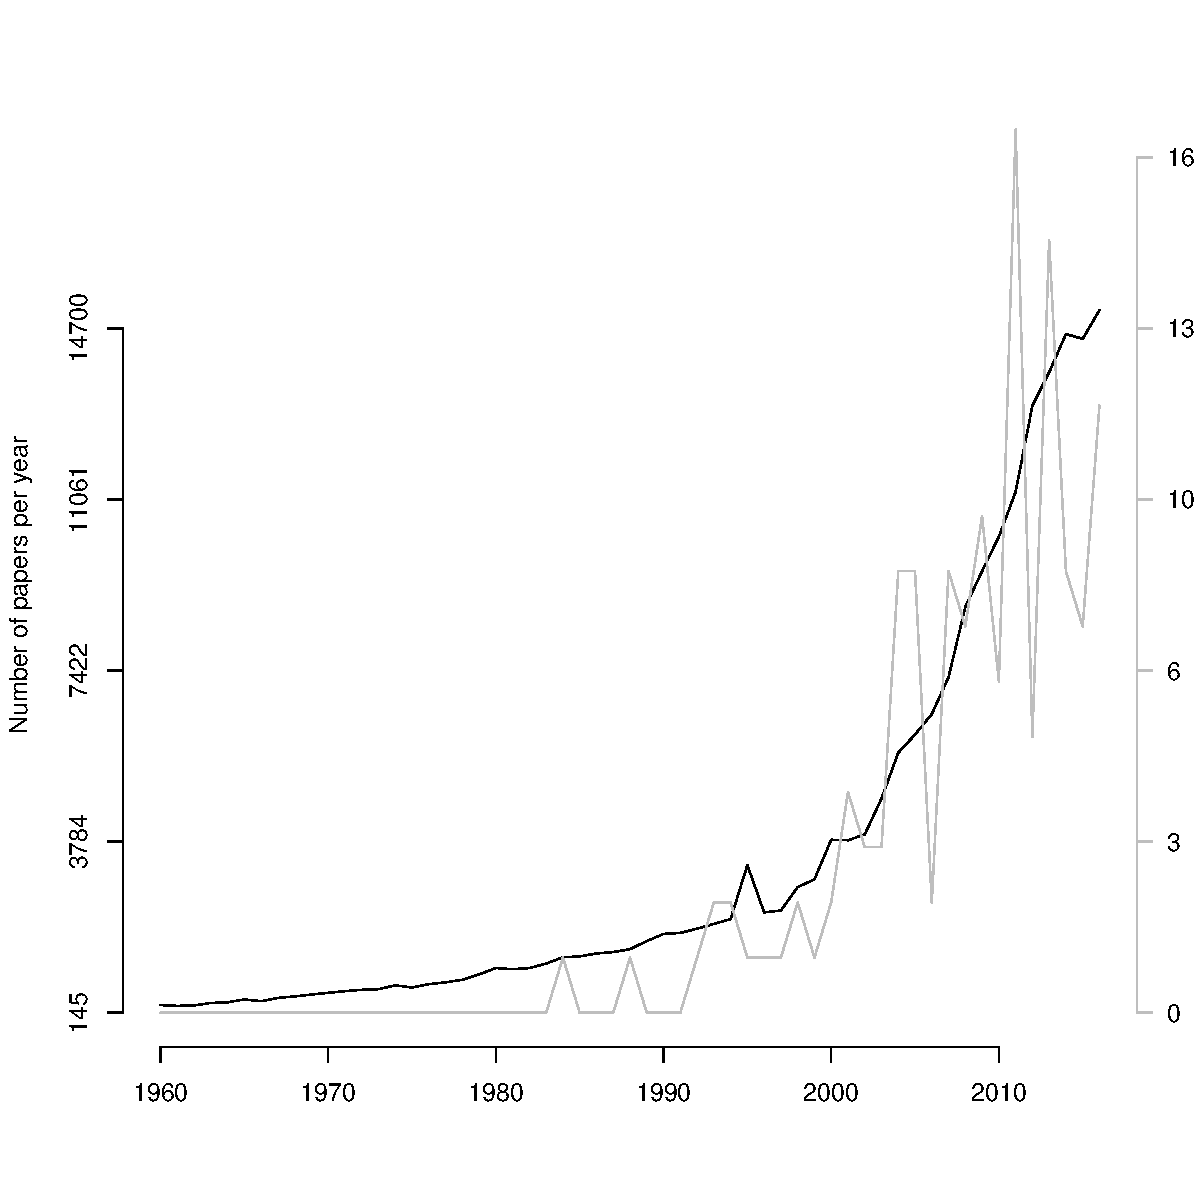
\includegraphics[width=1\textwidth]{Figures/GoogleScholarOccurences.pdf} 
% \caption{Number of papers on Google Scholar matching the search ``morphological disparity'' per year. In black, the match is in the paper and in grey, in the title. We collected the number of matches per year from 1960 to 2016 in Google Scholar for the terms "morphological disparity" both in the text (fuzzy matching) or in the title (exact matching). The data was collected on the 1st of November 2017.}
% \label{Fig:GoogleOccurences}
% \end{figure}


% \section{What actually \textit{is} disparity?}

% \cite{prentice2011} define disparity as: ``a term widely (albeit not always consistently) used to describe the range of forms in a group of organisms, or the difference among different body plans''.
% Disparity can describe either the metric (\citealt{Wills2001}; or index \citealt{Hopkins2017}) or the whole pipeline \citep{zelditch2012geometric,lloyd2016estimating}.
% To assess the usage of disparity in different published studies, we collected methodological data from the 500 first Google Scholar results for the key words ``morphological disparity'' per order of appearance (accessed on the 1st of November 2017).
% For the 230 relevant papers among the 500 matches, we collected the following methodological data: (1) What was the focal biological group? ; (2) What kind of data was measured (e.g. landmarks, discrete data, etc.)?  ; (3) Was data collected on the full organism or not? ; (4) How was the morphospace explicitly defined (e.g. PCA, PCO, MDS, etc.)? ; (5) How was the disparity metric(s) explicitly defined? ; (6) Which statistical test was applied to test the disparity related hypothesis? ; (7) Was phylogeny taken into account or not?
% We used only the explicit definition of the morphospace and the disparity metric(s) in this search since a few number of papers had a vague definition of either or both (e.g. a disparity metric was measured but not described anywhere in the paper).
% The remaining 270 matches were disparity was mentioned but not measured felt in the following categories: papers out of topic, papers mentioning morphological disparity without measuring it, review papers, papers not accessible (either through a broken link or a paywall) or referenced citation without the paper (as a Google Scholar match).
% To reduce the amount of categories for the 230 recorded methods, we concatenated different methods in a smaller number of categories (see supplementary materials and \url{https://github.com/TGuillerme/Disparity_Working_Group/blob/master/Analysis/data_cleaning.Rmd}).

% \begin{figure}[!htbp]
% \centering
%    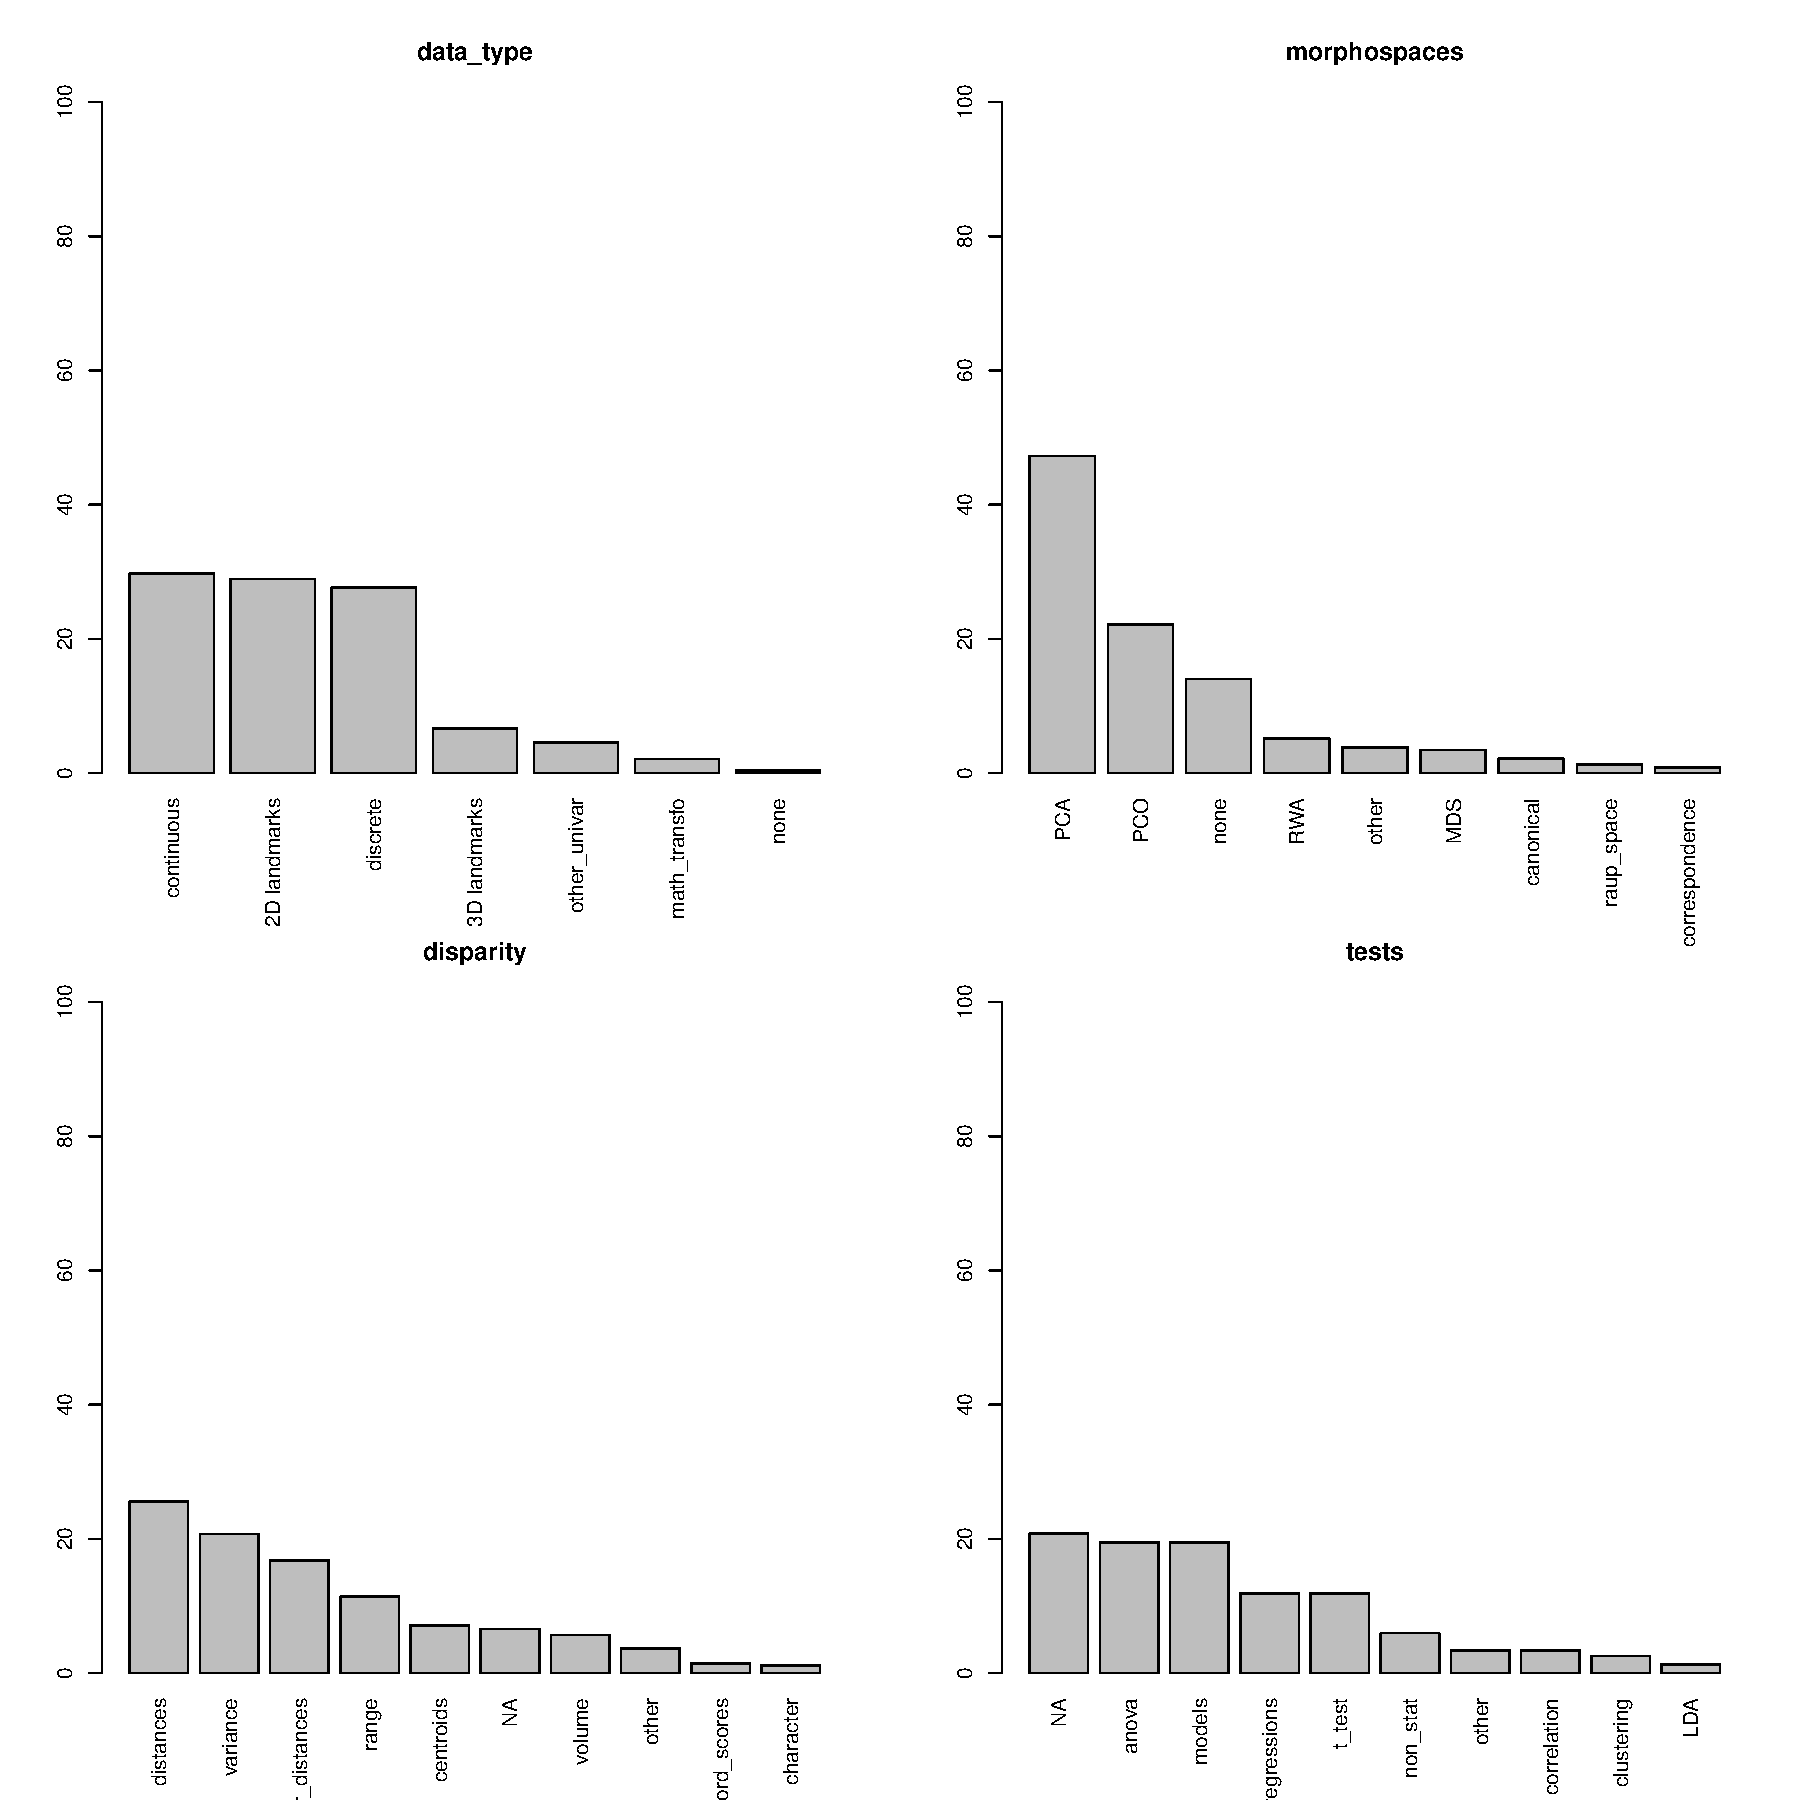
\includegraphics[width=1\textwidth]{Figures/MethodsProportions.pdf} 
% \caption{Disparity methods proportional usage: (1) Data type: which input data was used (...); (2) Morphospace: how was the morphospace obtained (...); (3) disparity: what type of disparity metric was calculated (...); (4) test: what type of test was applied (...).}
% \label{Fig:MethodsProportions}
% \end{figure}

% From the collected data, we can highlight the use of three main different disparity analysis with their associated data/morphospace/metric/tests and related to specific methodological implementations.

% \begin{itemize}
%     \item \textbf{The ``\texttt{Claddis}'' approach:} this group of methods uses discrete morphological data (sometimes referred to as ``Cladistic'' characters) for the full organisms to build a PCO from the organism's pairwise distance as a morphospace. Disparity is then often measured as a variation of the ordinated matrix dimensions' variances or ranges (e.g. the sum of variance or/and the sum of ranges). Hypothesis are often tested using multivariate ANOVAs on the pairwise distance matrix or by simply comparing the confidence intervals overlap of the disparity from different groups. 

%     \item \textbf{The ``\texttt{geomorph}'' approach:} this group of method is based on landmark data (2D or 3D) on parts of the organism studied usually the skull) and use a Procrustes transformation of the landmarks that are then directly ordinated using a PCA (but sometimes RWA). Disparity is often measured as a distance metric (e.g. the distance between the species and a point in the morphospace such as its centroid). Hypothesis are then tested using ANOVA type tests with usually no phylogenetic correction (although phylogeny is sometimes used to correct the morphospace).

%     \item \textbf{The ``\texttt{approach}'' approach:} this method can directly use continuous or discrete data for the full organism without any ordination (but not necessarily), and will measure disparity as the average pairwise distance between species (whether euclidean or any other type of distance). Hypothesis of higher/lower disparity can then be measured using null evolutionary models.
% \end{itemize}

% %
% The advent of these three approaches coincides with the explosion of disparity analysis (Fig. \ref{Fig:GoogleOccurences}) and suggest a high popularity of disparity analysis.
% %
% Unfortunately, however, few actual tests have been performed on whether any of these approaches \textit{actually} allows to tackle the classic disparity questions (see \ref{text:intro}{Introduction}).
% Are all these methods the right tools to answer these questions are they mere ``inductive fishing trips'' used to describe the data rather than testing any of the hypothesis related to the disparity questions?

% \section{Does data used in disparity analysis allows to test hypothesis?}
% In fact, the question of which data to analyse \citep{hetherington2015cladistic} and which part of the data to use has been analysed \citep{hopkins2017well} has rarely been assessed.
% Can the data used in disparity studies actually test the phenomenon researchers are trying to capture?

% For example, when studying discrete morphological characters (often following the ``\texttt{Claddis}'' approach), the data used is often recycled data used for phylogenetic analysis.
% These datasets are usually design to recover evolutionary history and differentiate clades and, often due to the preservations of the fossil record, are mainly based on hard tissue characters.
% In phylogenetics, this artefact have been shown to be leading to measurable topological recovery error (for soft \textit{vs} hard characters; \citealt{sansomfossilization2013}; or dental \textit{vs} cranial characters \citealt{sansom2017dental}).
% Therefore, is the morphospace composed of ``fossilisable'' characters enough for answering evolutionary hypothesis?
% For example, are niche replacement hypothesis equivalent to fossilisable-character-based-niches replacement hypothesis?

% Similarly, many studies in geometric morphometric are based solely on skull shape using landmark techniques combined with Procrustes superimposition \citep[the ``\texttt{geomorph}'' approach;][]{zelditch2012geometric,adams2017geometric}.
% However, it has been shown that the whole skeleton displays different integrated modules with different specific evolutionary constraints leading to variable rates and modes of evolution (\citealt{Goswami20130254}; and this even at the cranial level \citealt{goswami2010influence}).
% Is skull variation enough for measuring body plans variation through time for example?

% In the case where disparity is measured a single continuous trait (or a collection of traits; following the ``\texttt{geiger}'' approach), for example in \cite{price2014niche}, beak and limb length as well as body mass are used to differentiate groups of birds and different zones in the morphospace can then be interpreted as different niches.
% Is this set of traits studied in isolation sufficient to test niche occupancy hypothesis?

% Additionally, in many cases, the disparity metrics and hypothesis are often based on a transformation of the data (pairwise distances, PCA, PCO, MDS, RWA, etc.).
% Can these transformation readily reflect the raw data in our hypothesis?
% For examples a morphospace as a pairwise matrix reflects the dissimilarity between the data, a morphospace based on an ordination reflects the variability within the data, a morphospace based on both reflects the variability within the dissimilarity, are each method reflecting that?

% \section{Do the disparity metrics (or indices) really reflect variation in the studied phenomenon?}
% From the 230 papers analysed, we found 104 unique combination's of metrics to measure disparity (Fig. \ref{Fig:MethodsProportions}).
% Commonly, these metrics are used to approximate the volume occupancy within the morphospace \citep{Wills2001,DonohueDim,diaz2016global}.

% However, it has been shown that different metrics reacts differently depending on the dataset \citep[][; and an anecdotal example in Fig. \ref{Fig:DimensionsEffect}]{Wills2001,Ciampaglio2001}.
% For example metrics involving a product of aspects of the matrix (e.g. the volume, the product of the dimensions) are likely to suffer from the \textit{Curse of dimensionality} \citep{bellman1957dynamic} and will quickly tend to null values.
% Some other metrics are not representing all the data captured in the morphospace (e.g. the sum or product of variance ignores the co-variance between dimensions).
% Are these metrics as a description of the ordination a good proxy for the observed biological phenomenon?


% \begin{figure}[!htbp]
% \centering
%    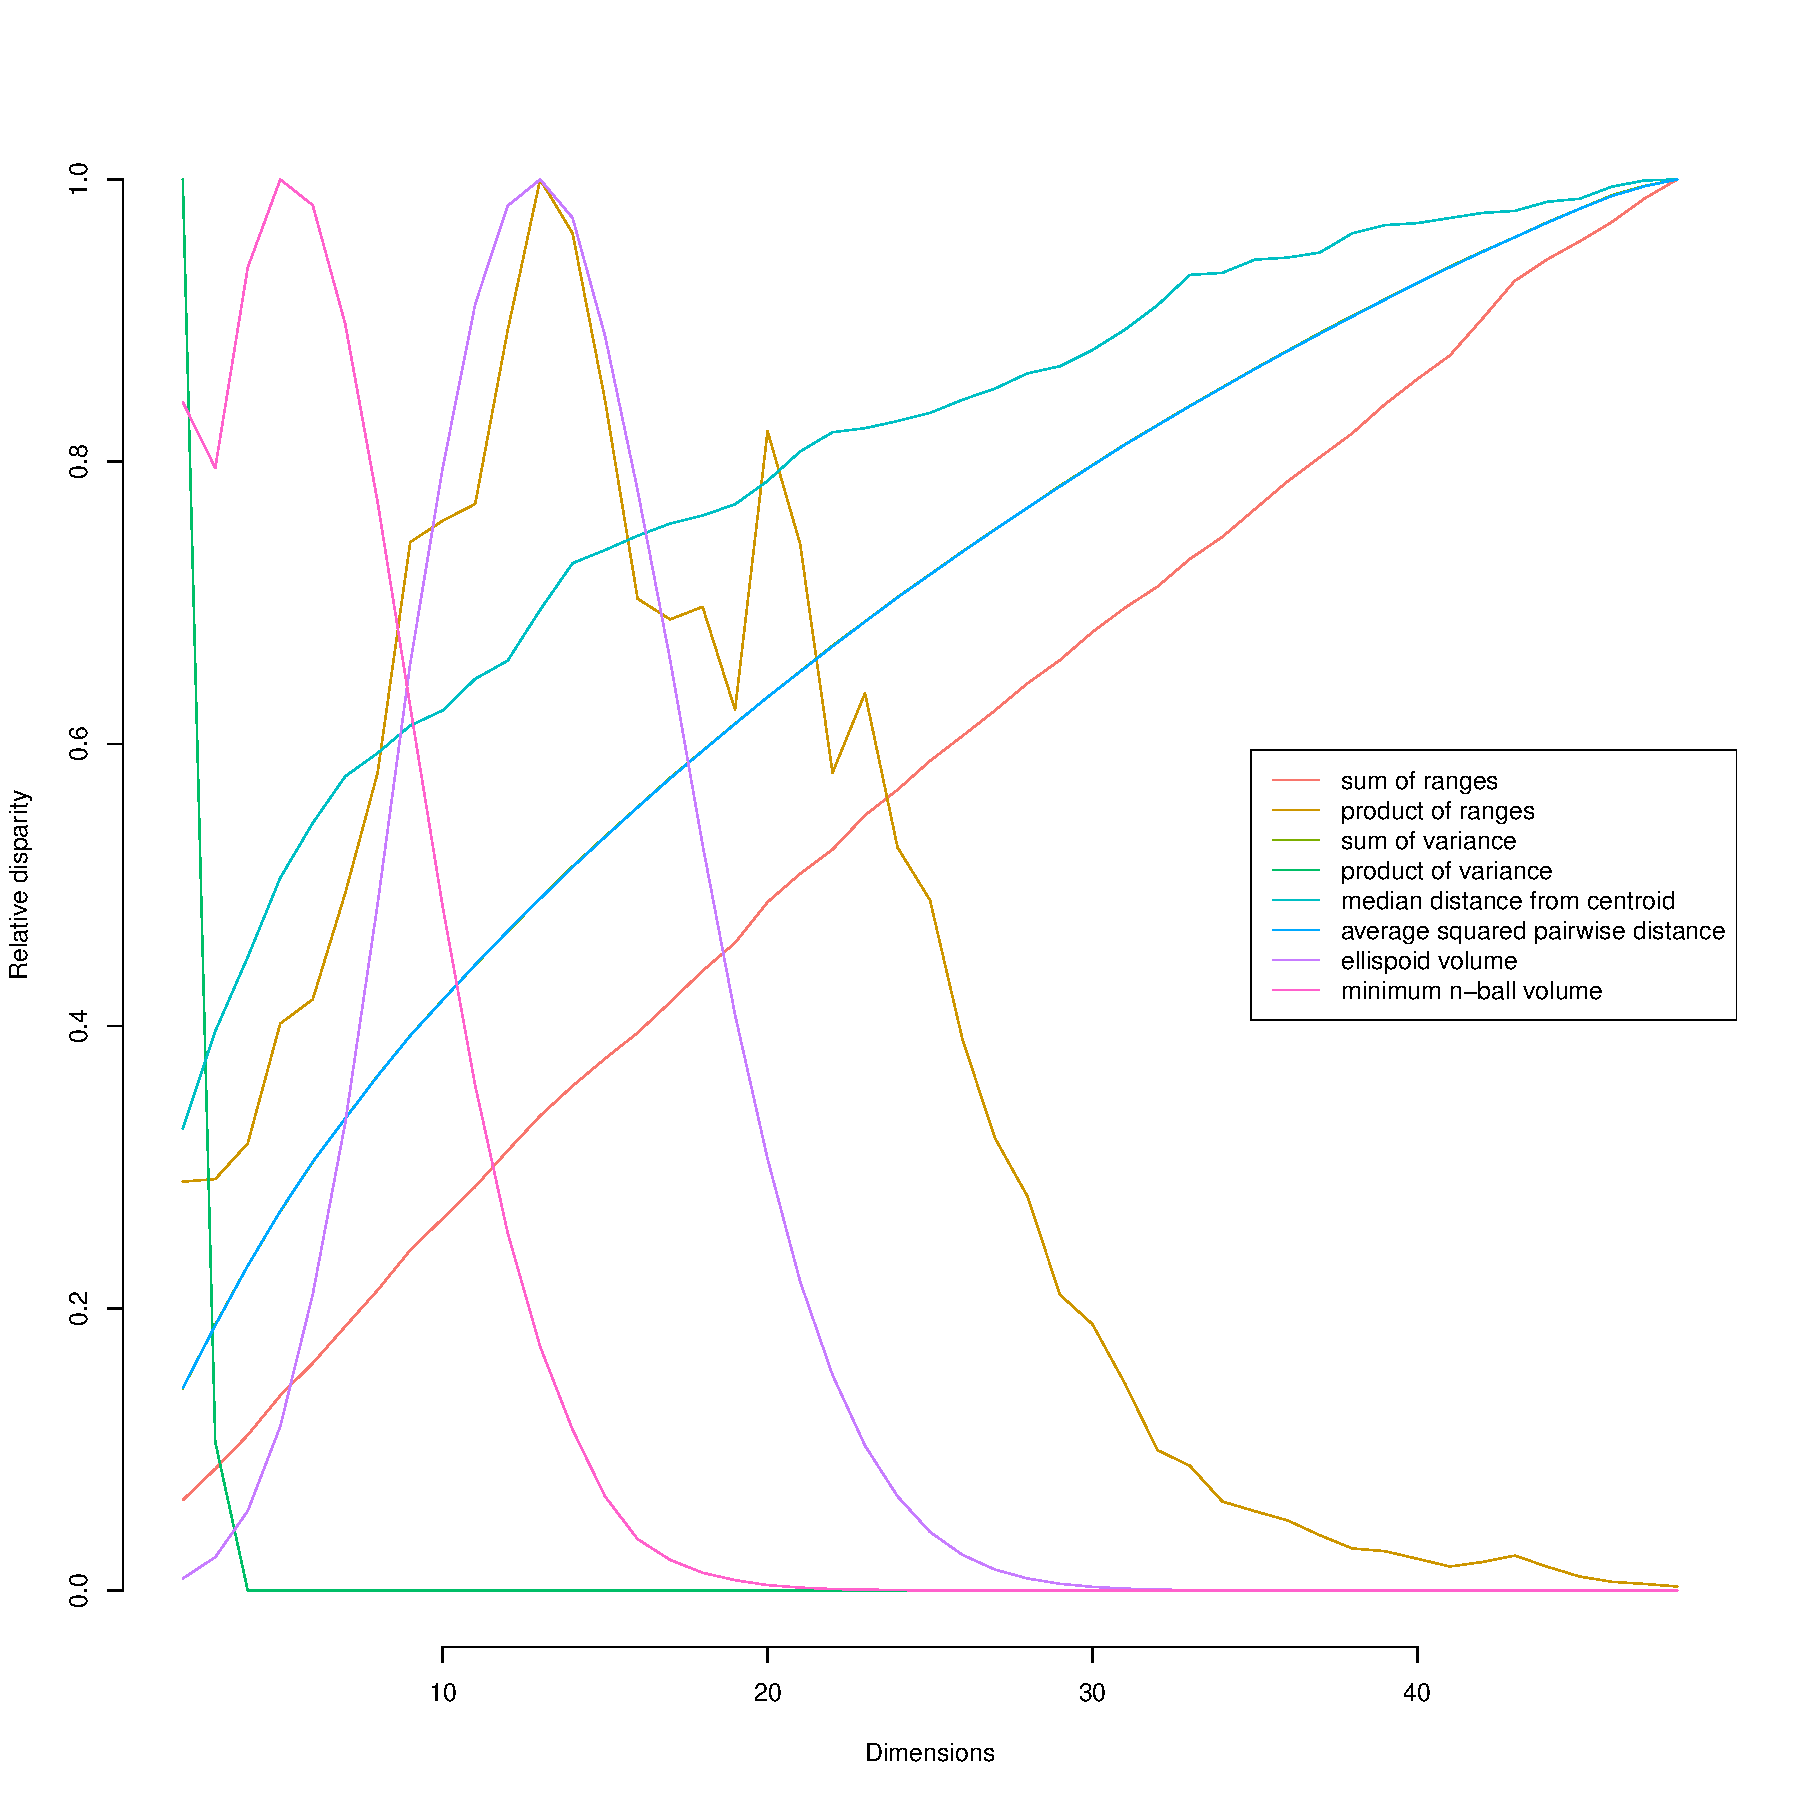
\includegraphics[width=1\textwidth]{Figures/DimensionsEffect.pdf} 
% \caption{Effect of the number of dimensions on different disparity metrics (note that the sum of variance is equal to the average squared pairwise distance in this case).
% The data used is one of the example datasets from the \texttt{dispRity R} package \citep[\texttt{BeckLee\_mat50};][]{beckancient2014,dispRityv02} composed of 50 elements and 48 dimensions obtained from a ordination (MDS) of the distance matrix of a discrete morphological character matrix.}
% \label{Fig:DimensionsEffect}
% \end{figure}

% Despite these caveats, it is important to actually know what the metrics are measuring.
% There has been some attempts to test that through simulations \citep{Ciampaglio2001,  gerber2017geometry} but it is still unclear which metric reflects the best the hypothesis test.
% For example, the average squared pairwise distance (or the sum of ranges) are really popular \citep[e.g.][]{geiger2008} yet has been shown to be fairly senstive, at least in empirical data to the number of sampled taxa, the number of characters and the data completeness \citep[][; although effects were lesser in simulations]{Ciampaglio2001}.
% More fundamentally, the question arises whether one disparity metric could be sufficient to describe changes in disparity?
% Changes in multidimensions might not be readily grasped by unidimensional metrics!
% For example, a given taxonomic group might have the exact same volume as another one yet be in a complete different part of the morphospace \citep[or even overlap or not depending on the dimensions;][]{davis2012acanthodes,brusatte50}.
% In this case, it might more interesting to have multiple metrics (e.g. the position and the volume) [FABRE et. al in prep.] or to use distributions of metrics (e.g. what does the average distance between species or from a point really convey? Is the distribution not more interesting?).

% Maybe we need metrics that fit explicitly our hypothesis (or fit our hypothesis directly to the metric).
% For example, for competitive replacement, should we not measure whether group A occupies the same place as group B through time and whether that is due to competition or simply because any other place in the space cannot be occupied (and why are such spaces unoccupied)?


% \section{Is the current statistical toolkit sufficient for testing disparity hypothesis?}
% Are the methods used to test hypothesis in disparity actually testing what we think they're testing (problem of multidimensional hypothesis)
% What does an anova or related variance based test real infirm/confirms regarding the disparity questions?
% How do we deal with bootstrapped data and pseudo-replications?
% Can we realistically use univariate Gaussian models to test hypothesis based on multivariate, probably non-Gaussian data? \citep{blomberg2017beyond}

% Should be take phylogeny into account? \citep{polly2013phylogenetic}



% \section{What are we missing?}

% \subsection{Learning lessons from other fields}
% In ecology, disparity bears strong parallels with $\beta$-diversity in ecology (a measure of ecological communities (dis)similarity): one biological observation described by a vast array of metrics \citep{baselga2010partitioning, anderson2011navigating, donohue2016navigating}.

% \section{Conclusion}
% We need a more hypothesis driven way of analysing disparity.
% Disparity methods should be the tool for answering disparity hypothesis, not merely a description of the data.




% \hl{[ADD Biological group, full organism and phylogeny in the supplementary]}

% \noindent \hl{\textit{These points should be developed during the meeting}}


% \subsection{Disparity data}
% The data used for disparity methods comes from three main sources:
% \begin{itemize}
%     \item Continuous data such as limb or body measurements \citep{slaterCetacean}.
%     \item Discrete morphological characters \citep[sometimes referred to as ``Cladistic'' characters; ][]{Brusatte12092008}.
%     \item Geometric morphometric data which is generally the Procrustes transformation of 2D or 3D landmarks \citep{cooney2017mega}.
% \end{itemize}

% However, data was by far not limited to these three categories (e.g. colours \citealt{maia2013key}; metabolic rate \citealt{nespolo2016studying} or chemicals signal \citealt{garcia2017heterogeneous}).

% \subsection{Morphospaces}
% \begin{itemize}
%     \item PCAs [CITE].
%     \item PCOs [CITE]
%     \item Pairwise distance matrices \citep[no ordination; ][]{Harmon961}.
% \end{itemize}

% But also RWA [CITE] or Raup-spaces [CITE].

% \subsection{Disparity metrics}
% Throughout the 230 analysed papers, we found 103 unique combinations of metrics!

% \begin{itemize}
%     \item Distances measurements between species or from a certain point in the morphospace [CITE].
%     \item Ranges and variances of each axis of the morphospace \cite{Wills2001,Ciampaglio2001}
%     \item Distance between species based on the pairwise distance matrix (not the ordinations) [CITE].
% \end{itemize}

% But also metrics based on the volume [CITE], the characters dissimilarity [CITE] or the coordinates of some axis of the ordination [CITE]

% \subsection{Disparity hypothesis}
% Describing the many outputs (what and how is it tested):

% \begin{itemize}
%     \item Variance based (ANOVA, etc.) [CITE].
%     \item Correlation based [CITE].
%     \item Regression based (PGLS, etc.) [CITE].
% \end{itemize}

% But also discriminant analysis [CITE] and clustering [CITE].

% Of course some studies use a combination of these three methods or none of them at all!

% Also, among each category XX\% of studies use multiple approaches.

% [ADD Biological group, full organism and phylogeny in the supplementary]

% \section{Expanding disparity}

% How to compare disparity between groups? Is disparity relative?

% How to compare disparity between methods?

% Can we really say things about competition when looking at disparity in a single group?

% Are all characters equal? Character contingency suggests otherwise

% What is the relationship between disparity and tree shape?

% Do we have a null model for investigating disparity?

% Can we really say things about competition when looking at disparity in a single group?


% \noindent \hl{\textit{Disparity in other fields}}

% In ecology, disparity bears strong parallels with $\beta$-diversity in ecology (a measure of ecological communities (dis)similarity): one biological observation described by a vast array of metrics \citep{baselga2010partitioning, anderson2011navigating, donohue2016navigating}.

% \section{Conclusion}

% A quick guideline for good disparity analysis:

% Maybe we need something like in Parham et al 2012 (Best Practices for Justifying Fossil Calibrations): an easy an identifiable description of the pipeline containing: 1) the type of data, 2) the morphospace and 3) the metric? 

\section{Acknowledgments}
The Royal Society.
TG acknowledge support from European Research Council under the European Union's Seventh Framework Programme (FP/2007 – 2013)/ERC Grant Agreement number 311092 awarded to Martin D. Brazeau.


\bibliographystyle{sysbio}
\bibliography{References}

\end{document}

